%% Template for MLP Coursework 1 / 16 October 2017 

%% Based on  LaTeX template for ICML 2017 - example_paper.tex at 
%%  https://2017.icml.cc/Conferences/2017/StyleAuthorInstructions

\documentclass{article}

\usepackage[T1]{fontenc}
\usepackage{amssymb,amsmath}
\usepackage{txfonts}
\usepackage{microtype}
\usepackage{enumitem}

% For figures
\usepackage{graphicx}
\usepackage{subfigure} 

% For citations
\usepackage{natbib}

% For algorithms
\usepackage{algorithm}
\usepackage{algorithmic}

% the hyperref package is used to produce hyperlinks in the
% resulting PDF.  If this breaks your system, please commend out the
% following usepackage line and replace \usepackage{mlp2017} with
% \usepackage[nohyperref]{mlp2017} below.
\usepackage{hyperref}
\usepackage{url}
\urlstyle{same}

% Packages hyperref and algorithmic misbehave sometimes.  We can fix
% this with the following command.
\newcommand{\theHalgorithm}{\arabic{algorithm}}


% Set up MLP coursework style (based on ICML style)
\usepackage{mlp2017}
\mlptitlerunning{MLP Coursework 4 (\studentNumber)}
\bibliographystyle{icml2017}

\DeclareMathOperator{\softmax}{softmax}
\DeclareMathOperator{\sigmoid}{sigmoid}
\DeclareMathOperator{\sgn}{sgn}
\DeclareMathOperator{\relu}{relu}
\DeclareMathOperator{\lrelu}{lrelu}
\DeclareMathOperator{\elu}{elu}
\DeclareMathOperator{\selu}{selu}
\DeclareMathOperator{\maxout}{maxout}

%% You probably do not need to change anything above this comment

%% REPLACE this with your student number
\def\studentNumber{s1700260, s1457374, s1784849}

\begin{document} 

\twocolumn[
\mlptitle{MLP Coursework 4: Project Final Report \\
Transfer learning and dataset size\\
Group G74
}

\centerline{\studentNumber}

\vskip 7mm
]

\begin{abstract} 
Write This Last.
\end{abstract} 

\section{Introduction}
\label{sec:intro}

Large-scale neural networks have become increasingly prevalent in artificial intelligence [INSERT REFERENCE HERE]. Such architectures effectively solve computer vision problems that were previously considered difficult to address using traditional symbolic manipulation [INSERT REFERENCE HERE]. One concern with modern neural networks is that their performance scales with the quantity of data used to train them, as demonstrated in our previous piece of research [INSERT REFERENCE HERE]. This concern is a problem for individuals or institutions with small amounts of data that want to implement these architectures as solutions, or for research purposes.

Data driven techniques exist, such as data augmentation [INSERT REFERENCE HERE], which help solve this problem [footnote: see our previous paper for a further explanation]. However, to draw from our previous research [INSERT REFERENCE HERE] we investigate alternative, machine learning based approaches, specifically transfer learning [INSERT REFERENCE HERE] as a method to improve the performance of neural network architectures that utilise small amounts of data. These techniques allow us to use the knowledge that a given (pre-trained) network already has and adapt the architecture to suit our requirements [INSERT REFERENCE HERE].

The objective of transfer learning is to use the knowledge acquired by an existing network that was built to solve a similar task and improve the generalization. The main idea is to try to adapt that previous knowledge to the new problem to be solved. One of the advantages of this technique is that the solution for the new problem does not have to start from scratch. Prior work can be re-utilised which is important when the resources are limited. This situation is specially true for convolutional neural networks which, depending on the size of the architecture, can require an important amount of computational power.

There exist a number of pre-trained neural networks to solve classification tasks in the field of computer vision. One of them is the Visual Geometry Group network (VGG net)[INSERT REFERENCE HERE]. This network implements a simple yet deep architecture with several convolutional layers. There are several configurations that vary the number of convolutional layers among 11, 13, 16, and 19. In every configuration the architecture includes maximum pooling layers of dimensions 2x2 and stride 1. The convolutions are performed using 3x3 filters with stride and pad of 1. Finally, ReLU activations after each convolution are utilised.

VGG net was firs used in the ImageNet Challenge 2014[INSERT REFERENCE HERE], which means that is was originally trained using the Imagenet dataset [INSERT REFERENCE HERE]. However, the network has also been trained in other datasets like CIFAR-10 [INSERT REFERENCE HERE] and CIFAR-100[INSERT REFERENCE HERE]. It is important to make this distinction since each dataset has been developed for a different purpose, therefore, they have specific characteristics. The knowledge learnt from a network depends on the dataset used to train it. Thus, it is critical to know the characteristics of the dataset utilised to train the network since it will play and important role when implementing transfer learning.

ImageNet is a large-scale hierarchical image database [INSERT REFERENCE HERE]. The structure of this dataset contains 12 main groups or sub-trees. Each sub-tree contains a variable number of categories. The total number of categories is 5247, each one containing on average 600 images; thus, the total number of images in the dataset is 3.2 million. As described, ImageNet is a large and diverse dataset. However, the original version of VGG net was trained on a subset of Imagenet that contains only 1000 categories using 1.3 million images for training, 50K images for validation and 100K images for testing.



\subsection{Interim Report Findings}
\label{sec:findings}

The research questions offered within this report have been drawn from our initial findings, as documented in the interim report [INSERT REFERENCE HERE]. To aid in orientating the reader, we provide a summary of these findings here.

It was possible to demonstrate how the amount of available data impacts the performance of a convolutional neural network. Such impact was observed in the validation stage by analysing the accuracy and error of the network. In the first case, it was evident the reduction of the accuracy as the size of the dataset was reduced. In the second case, the size of the dataset directly affected the error; the smaller the dataset, the bigger the error. In both cases, the ultimate effect of such behaviour was the difficulty of the network to generalize when the amount of data is small.

Futhermore, the usage of two different but comparable databases provided some extra insights about the behaviour of the neural network. In this case the observed accuracies in the validation stage were different for each dataset in every size used to train the network. Under these circumstances, it was clear that the dataset that allowed a higher accuracy (clothes) was less challenging for the network. This means, that the features extracted by the network were more useful and relevant for one of the datasets. In the other hand, the features learned by the network did not provide enough information to reach better results for the second dataset (expressions).

Finally, we demonstrated that a simple data driven technique like data augmentation effectively improves the performance of a simple convolutional neural network. However, the benefits of this method have a limit above which no further improvement can be done. All of these findings provided the foundations and motivation for our investigation.

\section{Objectives and Research Questions}
\label{sec:obj_questions}

\subsection{Objectives}
\label{sec:objectives}

The research presented within this report pertains to two fundamental objectives. The first one concerns with improving the performance of image classification tasks using transfer learning with limited amounts of data. The second objective investigates the generalisability of the methods as mentioned above to two distinctly different datasets [REF: APPENDIX: PARAGRAPH ON DATASETS]. Furthermore, we intend to propose and utilise a framework for measuring the similarity between datasets using a modified siamese neural network [INSERT REFERENCE HERE] architecture.

\subsection{Research Questions}
\label{sec:questions}
Following from the conclusions drawn from our interim report, our research questions are listed below.

\begin{enumerate}
  \item How much the performance for a given classification task can be improved by using transfer learning?  
  \item How much the application of transfer learning affect two distinct but comparable datasets?
\end{enumerate}

[INSERT RESEARCH QUESTIONS ABOUT ONE SHOT LEARNING]

\subsection{Hypotheses}
\label{sec:hypotheses}
\begin{enumerate}[label=\textbf{H.\arabic*}]
  \item \label{h:1} Transfer learning will provide a performance benefit with respect to the generalisability (measured through validation accuracy) for a given classification with small data.
  \item \label{h:2} Transfer learning will provide a larger performance boost when the size of the dataset used to initially train the model is small rather than large.
 \end{enumerate}

Within the remainder of this report a section that outlines the methodologies utilised to conduct our research [INSERT SECTION REFERENCE] is initially given. Thereafter, all experimental results are presented [INSERT SECTION REFERENCE] and a review of related work is provided [INSERT SECTION REFERENCE]. Finally, a set of conclusions are drawn [INSERT SECTION REFERENCE].

\section{Methodology}
\label{sec:methodology}

A discussion of the methodologies used to conduct our experiments is provided herein. These methodologies include all selected data structures and algorithms.

\subsection{Transfer Learning}
\label{sec:transferlearninng}

\subsubsection{\textbf{Chosen Transfer Model}}

We decided to select the VGG net configuration with 16 convolutional layers (hereinafter referred as VGG16) to transfer its knowledge into the clothes and expressions datasets. As previously mentioned this network is quite simple and deep, thus, the expectation is that the knowledge contained in this network will be good enough to increase the generalisability of the classification tasks using both datasets.

Since VGG16 has been trained in different datasets, we decided to use the knowledge obtained from ImageNet rather than other options like CIFAR-100. The main reason for this is the number of classes from the subset of ImageNet to train the network (1000) which is much bigger than the number of classes from CIFAR-100. The expectation is that the knowledge from ImageNet is wider, therefore it can provide better results when when transferring that knowledge into new datasets. 

\subsubsection{\textbf{Data Structure and Learning Algorithm}}

To conduct our experiments, a modification of the fully connected layers is made to adapt the model to our needs. This pipeline has a bottleneck between the convolutional layers and the fully connected ones. To reduce the impact of this bottleneck, we divide the process into two components.

Firstly, the fully connected layers are used to convert the raw images from the dataset to another representation. This representation is the output of the last convolutional layer. In some sense, this can be seen as an encoding process, where the network transitions from images that provide information about intensity, to images that provide other kinds of information. Simply put, we are converting the features from the raw images (pixels) to another feature space. The aforementioned process is time consuming, however, one of the benefits it provides is the dimensionality reduction. Input images are converted from 64x64 (4096) dimensional pixel vectors (representative of features) to a 2048 dimensional feature space that cannot be obviously identified or described. Once we have finished this process, we use the output to feed the fully connected layers.

Secondly, an adaption to the fully connected layers is required, we define three alternatives. The main difference each alternative is the number of fully connected layers utilised within the architecture. In the first option, we use one fully connected layer, which provides 205,607 parameters. The second alternative is to add another fully connected layer, leaving 210,307 parameters. The final alternative uses three fully connected layers, providing 211,407 parameters.

For the first fully connected layer we use the L2 regularisation strategy [INSERT REFERENCE HERE]. The main objective here is to avoid overfitting, which is especially important for small data. Each layer uses a uniform parameter initialisation strategy. [[This kind of initialisation allows to have the activation done in the linear part of a sigmoid function.]] For the output layer, a softmax activation with a categorical cross entropy error loss [INSERT REFERENCE HERE] is implemented. The implemented learning rule is Adam [INSERT REFERENCE HERE].

\subsection{One Shot Learning}
\label{sec:oneshot}

\subsubsection{\textbf{Siamese Neural Network}}

[[PLACEHOLDER]]

\subsubsection{\textbf{Algorithm}}

[[PLACEHOLDER]]

\section{Experiments}
\label{sec:experiments}

\subsection{Transfer Learning}

\subsubsection{\textbf{Motivation}}

[[TODO: Add additional objective]]

Within our set of experiments associated with transfer learning using the proposed methodology [INSERT SECTION REFERENCE HERE], we intend to measure the performance benefit that transfer learning provides. As it has already been established in our previous research that there is a reduction in model performance when the size of the dataset is reduced, our main focus is to measure the variability of benefit that transfer learning provides when using small data. Furthermore, we intend to conduct a manual sensitivity analysis in order to extract the optimal hyper-parameters from a pool of proposed values.

The aim of these experiments is to aid in providing a practical method of performing image classification tasks when there is limited available data to train, test and validate a model similar to our own.

\subsubsection{\textbf{Description}}

[[TODO: Tidy This Up]]

[[TODO: Mention The Seed Used and add a footnote to use the attached codebase to reproduce results.]]

[[TODO: Mention the fact that we're using two bloody datasets.]]

Following from our previous research, we concluded that a reduction in available data correlated to a reduction in model performance. As a result, we are concentrating on experiments using small data. Therefore, each experiment that was conducted used the following dataset sample sizes: 100\%, 10\%, 1\%, 0.1\%.

In order to search for a practical set of system parameters, we decided to also vary the activation function within the fully connected layers. Each experiment was initially performed using a standard sigmoid function [INSERT REFERENCE HERE] due to our initialisation strategy. However, we also ran each experiment using exponential linear units (ELU) [INSERT REFERENCE HERE] because this activation function enables non-linearities between layers. Moreover, ELU has a gradient that is similar to the natural gradient (smooth).

Finally, we also performed a manual sensitivity analysis by varying the learning rate values from the follow pool: 0.01, 0.001, 0.0001.

Based on the description of the components in the methodology for the transfer learning approach, we configured the experiment using three fully connected layers, two different types of activation function, four dataset subsamples and a pool of three different learning rates.

Combinations of the above result in 72 different experiments. Due to the amount of experiments and the limited computational resources, we set a fixed number of epochs for every experiment (20), and a fixed size for the mini-batches used for the stochastic gradient descent calculation (50).

After running the aforementioned experiments, we analysed the results based on the validation accuracy. Then, we selected the configurations that get the highest values for validation accuracy for dataset sizes of 1\% and 0.1\%. For further investigation we then perform new experiments with higher number of epochs to analyse the behaviour of the fully connected part of the architecture.

\subsubsection{\textbf{Results}}

[[TODO: Tidy This Up]]

In order to compare our results to baselines obtained in the previous report, we base our analysis of the transfer learning experiments on the validation accuracy.Overall, there is still an evident reduction of the performance of the architecture relate to the size of the datasets, as is shown in [figure X].

[INSERT FIGURE X HERE]

\begin{figure*}[tb]
    \vskip 5mm
        \begin{center}
            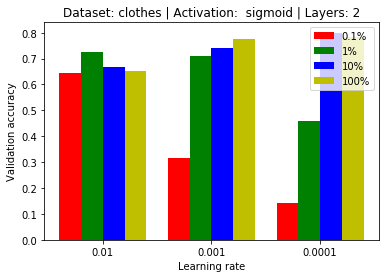
\includegraphics[scale=0.5]{accuracy_reduction_00.png}
            \caption{[[INSERT CAPTION HERE]]}
            \label{fig:2}
        \end{center}
    \vskip -5mm
\end{figure*}

\begin{figure*}[tb]
    \vskip 5mm
        \begin{center}
            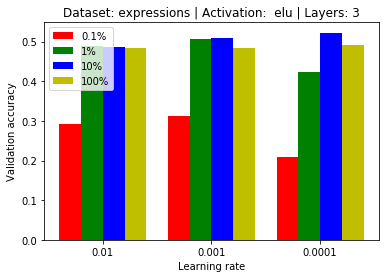
\includegraphics[scale=0.5]{accuracy_reduction_01.png}
            \caption{[[INSERT CAPTION HERE]]}
            \label{fig:3}
        \end{center}
    \vskip -5mm
\end{figure*}

For each dataset, the configuration that provides the highest accuracy for the smallest dataset size are quite different, as seen in \ref{tab:1}. It is specially important to note the activation functions. It is expected that the Sigmoid activation function gives better results since the uniform initialisation strategy is meant to benefit this activation function. However, in the case of expressions dataset, the best result is obtained with ELU, but the best accuracy using Sigmoid activations is not that far 0.30.

\begin{table*}[!htb]
  \centering
  \begin{tabular}{| l | l | l | l | l |}
    \hline
    \textbf{Dataset} & \textbf{Validation accuracy} & \textbf{Fully connected layers}& \textbf{Activation} & \textbf{Learning rates}\\ \hline
    Clothes & 0.64 & 2 & Sigmoid & 0.01 \\ \hline
    Expressions & 0.31  & 3 & ELU & 0.001 \\ \hline
  \end{tabular}
  \caption{Configuration that allows the highest accuracy for size of 0.1\% for clothes and expressions datasets}
  \label{tab:1}
\end{table*}

The proposed approach has provided more benefits to the clothes dataset than to the expressions one, as seen in \ref{fig:2} and \ref{fig:3}. This gives us some clues about the domain of the images in every dataset. Based on these results, we can say that the "distance" between the clothes domain and ImageNet domain is smaller than the "distance" between the expressions domain and ImageNet domain.

In comparison with the baseline system, it is clearly evident that the performance of the proposed system is better. For the clothes dataset reaches a performance similar to the one obtained using data augmentation. However, for the expressions dataset, the performance surpasses the one obtained with data augmentation. This might indicate that the conversion from the original feature space (pixel intensity) to the VGG16 feature space is more beneficial for the expressions than for the clothes.

\begin{table*}[!htb]
  \centering
  \begin{tabular}{| l | l | l | l | l |}
    \hline
    \textbf{Dataset} & \textbf{Baseline} & \textbf{Data Augmentation}& \textbf{Transfer learning} \\ \hline
    Clothes & 0.50 & 0.76 & 0.75 \\ \hline
    Expressions & 0.32  & 0.44 & 0.50 \\ \hline
  \end{tabular}
  \caption{Validation accuracy comparison between baseline system and approaches using data augmentation and transfer learning for size of 1\% for clothes and expressions datasets}
  \label{tab:2}
\end{table*}

\subsubsection{\textbf{Interpretation and Discussion}}

[[TODO: Tidy This Up]]

Observing the behaviour of the fully connected layers for the smallest sizes of both datasets, it is evident that the system is more stable for the clothes than for the expressions as seen in figure behaviour.png In the case of the clothes, for 1\% and 0.1\% of the original size, the system reaches a point where it starts to overfit. However, it is noticeable how the configuration of the system is robust enough to try to minimise this situation. The history is different for the expressions. Here, the behaviour is completely different not just compared to the clothes, but between the sizes of the dataset. In the case of the 1\% of the size, the configuration of the system is not robust enough to minimise the effect of overfitting. Once the overfitting starts, the system cannot make too much about it. However, for the case of 0.1\%, the configuration of the system is robust, not just to minimise the effects of overfitting, but to recover from it. This is not something immediate and it takes some time.

\subsection{Siamese Neural Network}

\subsubsection{\textbf{Motivation}}

[[PLACEHOLDER]]

\subsubsection{\textbf{Description}}

[[PLACEHOLDER]]

\subsubsection{\textbf{Results}}

[[PLACEHOLDER]]

\subsubsection{\textbf{Interpretation and Discussion}}

[[PLACEHOLDER]]

\section{Related Work}

[[PLACEHOLDER]]

\section{Conclusions}
\label{sec:conclusions}

[[PLACEHOLDER]]

[[REFERENCES GO HERE]]

%\bibliographystyle{abbrv}
%\bibliography{biblo.bib}

\end{document}